\documentclass[notheorems,hyperref={bookmarks=true}]{beamer}
\usepackage[framesassubsections]{beamerprosper}
\hypersetup{pdfpagemode=FullScreen}
\usepackage[utf8]{vietnam}
\usepackage{mdframed}
\usepackage[english]{babel}
\usepackage{ulem} %for underlying+
\usepackage{pifont} %for creating dingautolist
\usepackage[mathscr]{eucal}
\usepackage{amsfonts,amsmath, amsthm, amssymb,amsxtra,latexsym,amscd,graphics,graphpap}
\usepackage{indentfirst}
\usepackage{rotating}
\usepackage{graphicx}
\usepackage{amsbsy}
\usepackage{epsfig}
\usepackage{natbib}
\usepackage{cases} 

\usepackage{pdfpages}
\usepackage{multicol}
\usepackage{hyperref}
\usepackage{subfigure}
\usepackage{multimedia}
\usepackage{boxedminipage}
\usepackage{tikz}
\usepackage{nicefrac}
\setbeamertemplate{theorems}[numbered] % Đánh số định lý.
\usetheme{Boadilla} % puts title, section, etc on top

\usecolortheme{rose} 
\usefonttheme[onlylarge]{structurebold}
\usefonttheme{professionalfonts}
\setbeamercolor{title}{fg=red!80!black,bg=blue!20!white}
\setbeamertemplate{section in head/foot shaded}[default][20]
\setbeamertemplate{subsection in head/foot shaded}[default][20]
\setbeamertemplate{navigation symbols}{}
\setbeamertemplate{blocks}[rounded][shadow=true]
\setbeamerfont{small}{size=\small}
\setbeamerfont{footnote}{size=\footnotesize}
\setbeamerfont{script}{size=\scriptsize}
\setbeamerfont{tiny}{size=\tiny}

\theoremstyle{plain}
\newcommand{\thedefinition}{\arabic{section}.\arabic{definition}}
\newcommand{\thelemma}{\arabic{section}.\arabic{lemma}}
\newcommand{\thetheorem}{\arabic{section}.\arabic{theorem}}
\renewcommand{\thetable}{\Roman{table}}

\mode<presentation>
\setbeamertemplate{navigation symbols}{} 

\usepackage{wrapfig}
\usepackage{multicol}
%\setbeamertemplate{footline}{\raisebox{-2.2ex}{\pgfuseimage{logo.png}}}

\title[{\makebox[.15\paperwidth]{VAR \& Holt-Winters in demand forecasting }}]{Mô hình VAR và Holt-Winters và ứng dụng trong bài toán dự đoán nhu cầu sản phẩm} 
\author[Group 1]{Group 1
\\
Tạ Duy Hải - 20206197\\
Nguyễn Văn Nghiêm - 20206206\\
Nguyễn Hoàng Sơn - 20206165} 
\date{Hanoi, 1/2024}

\renewcommand{\sfdefault}{cmss}
\renewcommand{\rmdefault}{cmr}
\renewcommand{\ttdefault}{cmtt}
\numberwithin{equation}{section}
\usepackage{array}
\usepackage{ragged2e}
\justifying
\usepackage{blindtext}
\usepackage{geometry}
 \geometry{
right = 5.5mm
 }
\renewcommand{\baselinestretch}{1.15}
\setlength{\parindent}{1.5em}
%\setlength{\parskip}{1em}
\DeclareMathOperator*{\argmin}{arg\,min}
\newtheorem{prop}{Proposition}
\usepackage{amsmath}
\newtheorem{definition}{Definition}
\newtheorem{theorem}{Theorem}
\newtheorem{corollary}{Corollary}
\newtheorem{hypothesis}{Hypothesis}
\usepackage{esvect}
\usepackage{booktabs}
\usepackage{multirow}
\begin{document}
	\begin{footnotesize}
		\begin{frame}
			\frametitle{}
			\maketitle
			%	\begin{block}
			%	\titlepage
			%	\end{block}
		\end{frame}
		
		\AtBeginSection[] % Do nothing for \section*
		{
			\begin{frame}<beamer>
				\frametitle{Outline}
				\tableofcontents[currentsection, currentsubsection]
			\end{frame}
		}
	\begin{frame}{Outline}
	    \tableofcontents
	\end{frame}	
\section{Giới thiệu bài toán}
\begin{frame}{Giới thiệu bài toán}
     Một trong những quyết định quan trọng nhất là quyết định
về sản xuất và cung ứng. Để đưa ra quyết định này một cách hiệu quả, doanh
nghiệp cần có một dự báo nhu cầu sản phẩm chính xác.

Những mô hình dự báo theo hướng học sâu thường được sử dụng có thể kể đến như ANN, LSTM, \dots Tuy nhiên, lớp mạng trên yêu cầu lượng lớn dữ liệu lịch sử trong quá trình huấn luyện để đạt được hiệu quả tốt nhất.

 Để đáp ứng với điều kiện thực tế thiếu thốn dữ liệu, các mô hình được chọn trong báo cáo này bao gồm: mô hình VAR và mô hình làm mượt Holt-Winters.
\end{frame}


\section{Mô hình VAR}
\begin{frame}{Mô hình VAR}
    Ta có chuỗi thời gian đa biến K chiều T quan sát $y_1,\dots,y_T$ với $y_t = (y_{1t}, \dots, y_{Kt})$ là quá trình dừng và công thức chung:
\begin{equation}
    y_t = \nu + A_1 y_{t-1} + \dots + A_p y_{t-p} + u_t. \label{ep:2.1}
\end{equation}

Với $\nu = (\nu_1, \dots, \nu_K)$ là vector hằng số $K \times 1$, $A_i$ là ma trận hệ số $K \times K$ và $u_t$ là nhiễu trắng với ma trận hiệp phương sai $\Sigma_u$.
\end{frame}

\begin{frame}{Phương pháp Ordinary Least Squares (OLS)}
    Phương pháp được trình bày bởi \text{Helmut L\"utkepohl} \footnote{\text{Helmut L\"utkepohl}, \textit{New Introduction to Multiple Time Series Analysis}, Springer Berlin, Heidelberg, 2005}. Ta định nghĩa:
    \begin{align*}
    & Y := (y_1, \dots, y_T) & (K \times T), \\    
    & B := (\nu, A_1, \dots, A_p) & (K \times (Kp + 1)), \\   
    & Z_t := [1, y_t, \dots, y_{t-p+1}]' &  ((Kp + 1) \times 1), \\
    & Z := (Z_0, \dots, Z_{T-1}) & ((Kp + 1) \times T), \\
    & U := (u_1,\dots, u_T) & (K \times T), \\
    & \textbf{y} := \text{vec}(Y) & (KT \times 1), \\
    & \beta := \text{vec}(B) & ((K^2p+K) \times 1), \\
    & \textbf{b} := \text{vec}(B') & ((K^2p+K) \times 1), \\
    & \textbf{u} := \text{vec}(U) & (KT \times 1). \\
\end{align*}
    
\end{frame}

\begin{frame}{Phương pháp Ordinary Least Squares (OLS)}
    Khi đó, công thức \ref{ep:2.1} được viết lại thành

\begin{equation}
    Y = BZ + U
\end{equation}

Khi đó, ta có: 
\begin{align}
        && \text{vec}(Y) &= \text{vec}(BZ) +\text{vec}(U) \nonumber \\  
       \Leftrightarrow && \text{vec}(Y) & = (Z' \otimes I_K) \text{vec}(B) + \text{vec}(U) \nonumber \\ 
        \Leftrightarrow && \textbf{y}  &= (Z' \otimes I_K) \beta + \textbf{u}. \label{eq:2.3}
\end{align}

\end{frame}

\begin{frame}{Phương pháp Ordinary Least Squares (OLS)}
Ta cần cực tiểu hàm sau để tìm được ước lượng cho $\beta$:

\begin{equation}
    S(\beta) = \textbf{u}' (I_T \otimes \Sigma_u)^{-1} \textbf{u}.
\end{equation}

Ta thu được nghiệm tối ưu:

\begin{equation}
    \hat{\beta} = ((ZZ')^{-1}Z \otimes I_K )\textbf{y}.
\end{equation}
\end{frame}

\begin{frame}{Phương pháp  Durbin-Levinson}
    Whittle (1963) và Robinson (1963) đã khái quát thuật toán Durbin - Levison cho trường hợp chuỗi thời gian đa biến\footnote{Jones. R. H.,  Multivariate autoregression estimation using residuals. \textit{In Applied Time Series Analysis I} (pp. 139-162). Academic Press, 1978.}.

    Ta có ma trận hiệp phương sai kích thước $K \times K$ với độ trễ $j$:
\begin{equation}
    \hat{R_j} = \frac{1}{n} \sum_{t = 1} ^{n-j} y_{t+j} y_t '.
\end{equation}
\end{frame}

\begin{frame}{Phương pháp  Durbin-Levinson}
    Chuỗi AR bậc $p$ có dự đoán tiến:

\begin{equation}
    \hat{y_t}^{(f)} = \sum_{k = 1}^p A_k^{(p)} y_{t-k},
\end{equation}

và dự đoán lùi:

\begin{equation}
    \hat{y_t}^{(b)} = \sum_{k=1}^p B_k^{(p)} y_{t+k}, 
\end{equation}

với $A_k^{(p)}$ và $B_k^{(p)}$ là ma trận $K \times K$. 
\end{frame}

\begin{frame}{Phương pháp  Durbin-Levinson}
    Giá trị khởi tạo:

\begin{equation}
    S_0^{(f)} = S_0^{(b)} = R_0
\end{equation}

Bước đầu tiên:

\begin{align}
    & A_1^{(1)} = R_1 \left[ S_0 ^{(b)} \right]^{-1} \\
    & B_1^{(1)} = R_{-1} \left[ S_0 ^{(f)} \right]^{-1}
\end{align}


với 
\[
    R_{-1} = R_1'
\]
\end{frame}

\begin{frame}{Phương pháp  Durbin-Levinson}
    Công thức chung:

\begin{align}
    & A_p^{(p)} = (R_p - \sum_{k=1}^{p-1} A_k^{(p-1)} R_{(p-k)} ) \left[ S_{(p-1)}^{(b)}\right]^{-1} \\
    & B_p^{(p)} = (R_p' - \sum_{k=1}^{p-1} B_k^{(p-1)} R'_{(p-k)} ) \left[ S_{(p-1)}^{(f)}\right]^{-1}
\end{align}

Công thức cập nhật ma trận:

\begin{align}
    & A_k^{(p)} = A_k^{(p-1)} - A_p^{(p)} B_{p-k}^{(p-1)} \\
     & B_k^{(p)} = B_k^{(p-1)} - B_p^{(p)} A_{p-k}^{(p-1)}
\end{align}
\end{frame}

\begin{frame}{Phương pháp  Durbin-Levinson}
    Dự báo 1 bước tiến và lùi của ma trận hiệp phương sai nhiễu:

\begin{align}
    & S_p^{(f)} = (I - A_p^{(p)} B_p^(p)) S_{p-1} ^{(f)} \\
    & S_p^{(b)} = (I - B_p^{(p)} A_p^(p)) S_{p-1} ^{(b)}
\end{align}
\end{frame}



\section{Mô hình làm mượt Holt-Winters}
\begin{frame}{Mô hình làm mượt Holt-Winters}
    Phương pháp Holt-Winters là một phương pháp dự báo chuỗi thời gian
mạnh mẽ được thiết kế để xử lý các chuỗi có tính xu hướng và tính mùa.

Trong phần này nhóm tác giả trình bày phương pháp Holt-Winters cộng tính và biến thể để sử dụng với chuỗi thời gian đa biến. 
\end{frame}

\begin{frame}{Mô hình làm mượt Holt-Winters}
       Xét chuỗi thời gian đơn biến $\textbf{y} = \left\{y_1, \dots, y_t\right\}$ với tính mùa có chu kỳ $p$. 
       
       Các quan sát này được biểu diễn dưới dạng $y_i = a_{i-1} + b_{i-1} + c_{i-1}, \ i= \overline{1, t}$, trong đó $a_i$ là thành phần mức độ, $b_i$ là phần xu thế và $c_i$ là phần mùa.
\end{frame}

\begin{frame}{Mô hình làm mượt Holt-Winters}
    Phương pháp cộng tính có $3$ phương trình làm mượt và một phương trình dự báo như sau:
    \begin{align} 
        &a_i = \alpha\left(y_i - c_{i-p}\right) + \left(1-\alpha\right)\left(a_{i-1} + b_{i-1}\right),\label{eq:3.1} \\
        &b_i = \beta\left(a_i - a_{i-1}\right) + \left(1 - \beta\right)b_{i-1}, \label{eq:3.2}\\
        &c_i = \gamma\left(y_i - a_{i-1} - b_{i-1}\right) + \left(1-\gamma\right)c_{i-p},\label{eq:3.3} \\
        &\hat{y}_{t+h \vert t} = a_t + h b_t + c_{t+h - p\left(k+1\right)}. \label{eq:3.4}
    \end{align}
    
\end{frame}

\begin{frame}{Mô hình làm mượt Holt-Winters}
    Bermúdez và các cộng sự \footnote{Bermúdez. J. D., Segura, J. V., \& Vercher, E. , Holt–Winters forecasting: an alternative formulation applied to UK air passenger data, \textit{Journal of Applied Statistics}, 34(9), 1075-1090, 2007.} đề xuất sử dụng mô hình hồi quy để ước lượng các tham số $\alpha, \beta, \gamma$ và giá trị ban đầu để thực hiện phương pháp cộng tính. Cụ thể các biến ngẫu nhiên $Y_i$ được biểu diễn dưới dạng
    \begin{align}
        Y_i = a_{i-1} + b_{i-1} + c_{i-1} +  \epsilon_i. \label{eq:3.5}
    \end{align}
    Trong đó $\epsilon_i \sim \mathcal{N}\left(0, \sigma^2\right)$.
\end{frame}


\begin{frame}{Mô hình làm mượt Holt-Winters}
    Kết hợp \ref{eq:3.5}, \ref{eq:3.1}, \ref{eq:3.2}, \ref{eq:3.3} thu được biểu diễn:

    \begin{align*}
        &Y_1 = a_0 + b_0 + c_{1-p} + \epsilon_1  \\
        &Y_2 = a_0 + 2b_0 + c_{2-p} + \alpha\left(1+\beta\right)\epsilon_1 +  \epsilon_2  \\
        & \vdots \\
        & Y_{p+1} = a_0 + \left(p + 1\right)b_0 + c_{1-p} + \gamma \epsilon_1 + \alpha \sum_{r= 1}^p \left(1 + \beta\left(p+1-r\right)\right)\epsilon_r + \epsilon_{p+1} \\
        &\dots
    \end{align*}
\end{frame}


\begin{frame}{Mô hình làm mượt Holt-Winters}
      Từ biểu diễn trên, tổng hợp lại thu được biểu diễn dạng ma trận
    \begin{align}
        \textbf{Y} = M \psi + L \epsilon         
    \end{align}
    
    Trong đó $\psi = \left(b_0, c_{1-p}, c_{2-p}, \dots, c_0\right)', a_0 = -b_0$ là véc tơ điều kiện ban đầu, $M$ là ma trận cỡ $t \times \left(p+1\right)$ với cột đầu tiên là $\left(0,1, \dots,t-1 \right)$ và $p$ cột còn lại được tạo bởi các ma trận đơn vị cỡ $p \times p$ xếp từ trên xuống dưới đủ $t$ hàng.  
\end{frame}

\begin{frame}{Mô hình làm mượt Holt-Winters}
     Ma trận $L$ có biểu diễn
    \begin{align}
        L = \begin{bmatrix}
        1 & 0 & 0 & \dots & 0  & 0\\
        l_2 & 1 & 0 & \dots & 0  & 0\\
        l_3 & l_2 & 1 & \dots & 0  &0\\
        \vdots& \vdots& \vdots& \ddots&\vdots &\vdots\\
        l_{n-1} & l_{n-2} & l_{n-3} & \dots& 1 & 0\\
        l_n& l_{n-1}& l_{n-2}&\dots&l_2&1
        \end{bmatrix}
    \end{align}
    
    với $l_i = \alpha\left(1 + \left(i-1\right)\beta\right) + \gamma\left(i = 1 \ \text{mod} \ p \right)$. $\epsilon = \left(\epsilon_1, \dots, \epsilon_t\right)$ là véc tơ nhiễu ngẫu nhiên độc lập cùng phân phối chuẩn.
\end{frame}


\begin{frame}{Mô hình làm mượt Holt-Winters}
    Hàm Log-Likelihood của $\textbf{Y}$ lúc này bằng
    \begin{align}
        -\dfrac{t}{2}\ln\left(\sigma^2\right) - \dfrac{1}{2\sigma^2} \left(\textbf{Y} - M \psi\right)'\left(LL'\right)^{-1}\left(\textbf{Y} - M \psi\right).
    \end{align}
    Các tham số $\alpha, \beta, \gamma$ được xác định bằng cực đại hàm hợp lý trên, tương đương với cực tiểu hóa
    \begin{align}
        \min_{\alpha, \beta, \gamma} \left(L^{-1} \textbf{Y}\right)' \left(I - P_X\right) L^{-1} \textbf{Y}.
    \end{align}
    
    Trong đó $X = L^{-1}M$ và $P_X = X \left(X'X\right)^{-1}X'$.
\end{frame}

\begin{frame}{Mô hình làm mượt Holt-Winters}
    Sau khi thu được $\alpha, \beta, \gamma$, ta sẽ tính lại $\hat{L}, \hat{X}$, từ đó ước lượng được véc tơ điều kiện ban đầu
    \begin{align}
        \hat{\psi} = \left(\hat{X}'\hat{X}\right)^{-1} \hat{X}'\hat{L}^{-1} \textbf{Y}.
    \end{align}
    
    Với bộ điều kiện ban đầu $\psi$, ta đã có thể sử dụng phương pháp cộng tính để tính các tham số và đưa ra dự báo. Lưu ý rằng mô hình trên hoạt động với chuỗi thời gian đơn biến.
\end{frame}

\begin{frame}{Mô hình làm mượt Holt-Winters}
    Xét chuỗi thời gian đa biến $\mathcal{Y} = \left(\textbf{Y}_1, \dots, \textbf{Y}_n\right) $ với $\textbf{Y}_i = \left(Y_{1i}, \dots, Y_{ti}\right)$. Để mô hình hồi quy trên áp dụng được, nhóm tác giả coi các véc tơ $\textbf{Y}_i$ đều có biểu diễn
    \begin{align}
        \textbf{Y}_i = M \psi + L \epsilon.  
    \end{align}
    
    Hay các chuỗi đều có chung bộ tham số $\alpha, \beta, \gamma$.
\end{frame}

\begin{frame}{Mô hình làm mượt Holt-Winters}
    Các tham số này được tìm bằng cách cực tiểu hóa
    \begin{align}
        \min_{\alpha, \beta, \gamma} \sum_{i=1}^n \left(L^{-1} \textbf{Y}_i\right)' \left(I - P_X\right) L^{-1} \textbf{Y}_i.        
    \end{align}
    
    Các ước lượng điều kiện ban đầu thu được bởi
    \begin{align}
        \hat{\psi}_i = \left(\hat{X}'\hat{X}\right)^{-1} \hat{X}'\hat{L}^{-1} \textbf{Y}_i.        
    \end{align}
\end{frame}

\begin{frame}{Mô hình làm mượt Holt-Winters}
        Ngoài ra nhóm tác giả còn đề xuất cách tìm $\alpha, \beta, \gamma$ thông qua cực tiểu hàm bình phương sai số
    \begin{align}
        \min_{\alpha, \beta,\gamma} \dfrac{\sum_{i=1}^n w_i \sum_{j=1}^t \left(Y_{ji} - \hat{Y}_{ji}\right)^2}{\sum_{i=1}^n w_i}.
    \end{align}
    Với $\hat{Y}_{ji} = a_{j-1, i} + b_{j-1,i} + c_{j-1,i}$.
\end{frame}
\section{Kết quả thực nghiệm}
\begin{frame}{Mô tả dữ liệu và bài toán}
    Trong báo cáo này, nhóm sử dụng bộ dữ liệu của một công ty do Giảng viên TS. Nguyễn Thị Ngọc Anh cung cấp. Bộ dữ liệu này gồm 2 file excel:
\begin{itemize}
    \item SP\_Plan: Kế hoạch bán sản phẩm A, B1, B2 trong 12 quý, từ 2021 đến 2023.
    \item SP\_DoiThu: Kế hoạch bán sản phẩm bao gồm cả lượng và giá trị của A, B, C trong 46 tháng, từ 1/2020 đến 10/2023.
\end{itemize}

Bài toán dự báo kế hoạch 1-4 quý tiếp theo của từng sản phẩm A, B1, B2.
    
\end{frame}

\begin{frame}{Mô tả dữ liệu và bài toán}
    \begin{figure}[H]
    \centering
    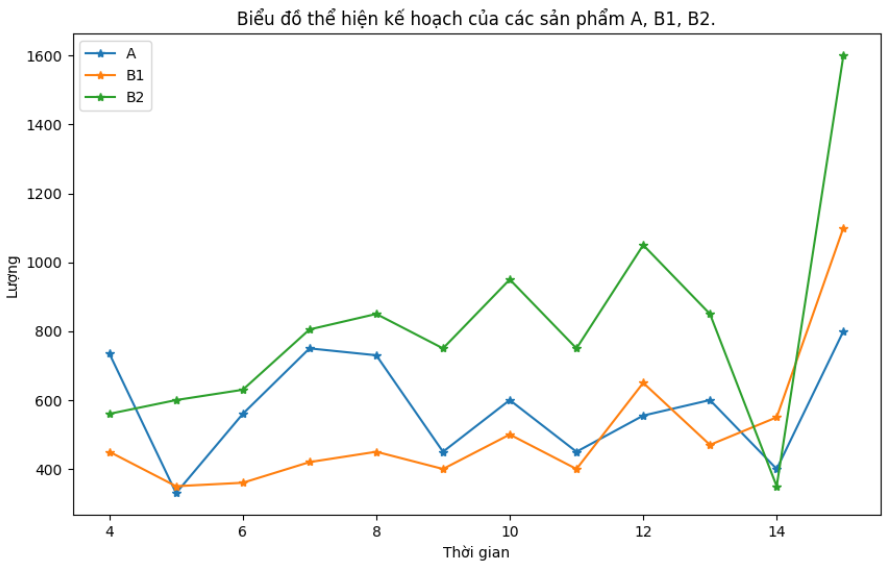
\includegraphics[width = 0.8\textwidth]{figure/AB1B2.png}
    \caption{Biểu đồ thể hiện số lượng của sản phẩm A, B1, B2 theo quý.}
    \label{fig:AB1B2}
\end{figure}
\end{frame}

\begin{frame}{Mô tả dữ liệu và bài toán}
    \begin{figure}[H]
    \centering
    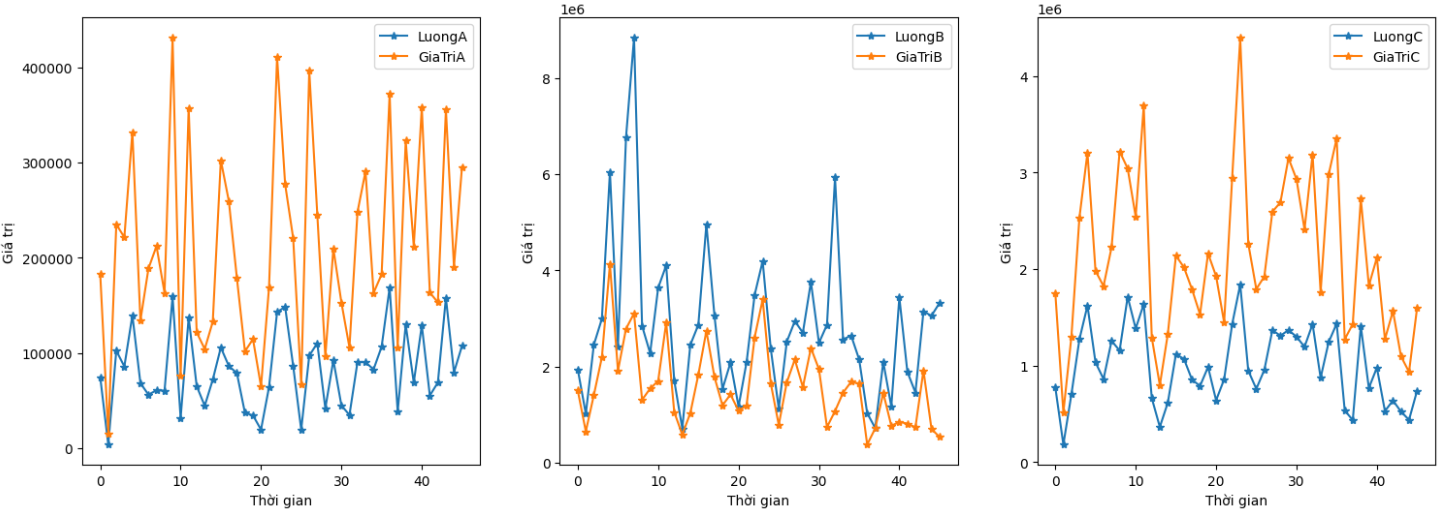
\includegraphics[width = 0.9\textwidth]{figure/ABCGiaTriLuong.PNG}
    \caption{Biểu đồ thể hiện sản phẩm A, B, C đối thủ theo tháng.}
    \label{fig:ABCGiaTriLuong}
\end{figure}
\end{frame}

\begin{frame}{Xử lý dữ liệu}
    Do kế hoạch bên công ty là theo quý, còn đối thủ là theo tháng. Do đó gộp 3 tháng làm 1 quý và bỏ đi phần kế hoạch năm 2020 và tháng 10/2023 của đối thủ, quý 4 năm 2023 của công ty. Bỏ đi kế hoạch của sản phẩm C, và chỉ lấy phần lượng của mỗi sản phẩm A, B. Còn lại thu được 11 quý từ quý 1/2021 đến quý 3/2023. 

    \begin{figure}[H]
    \centering
    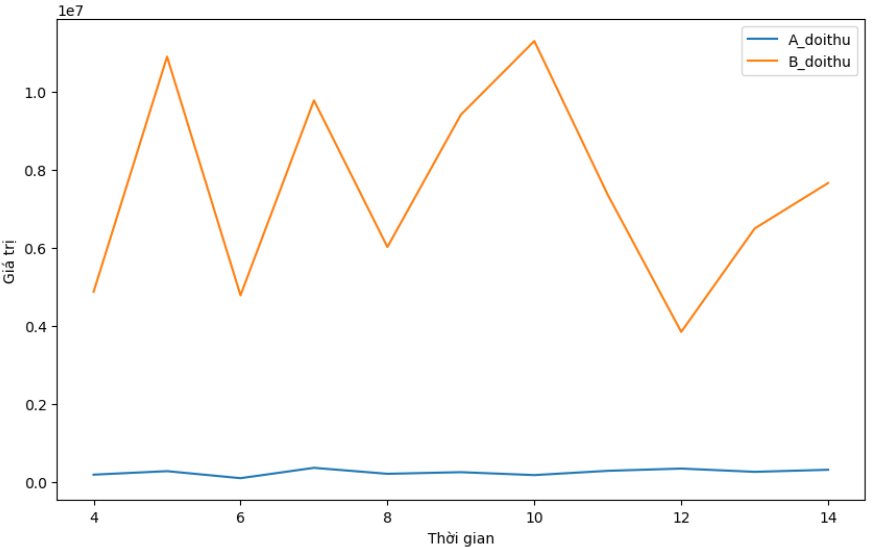
\includegraphics[width = 0.7\textwidth]{figure/ABLuong.PNG}
    \caption{Biểu đồ thể hiện sản phẩm A, B của đối thủ theo quý.}
    \label{fig:ABLuong}
\end{figure}

\end{frame}


\begin{frame}{Xây dựng mô hình}
    Nhóm chia dữ liệu thành 2 tập train và test với train gốm 7 quý đầu, test gồm 4 quý sau. Và xây dựng, thử nghiệm các mô hình sau:
\begin{itemize}
    \item Sử dụng với 2 trường A, A đối thủ: VAR - OLS, VAR - Durbin-Levinson.
    \item Sử dụng với 3 trường B1, B2, B đối thủ: VAR - OLS, VAR - Durbin-Levinson.
    \item Sử dụng 5 trường A, B1, B2, A đối thủ, B đối thủ: VAR - OLS, VAR - Durbin-Levinson, Holt-Winter tối ưu theo Log-Likelihood, Holt-Winters tối ưu theo MSE.
\end{itemize}
\end{frame}

\begin{frame}{Kết quả thực nghiệm}
    Qua quá trình thử nghiệm, nhóm sử dụng độ đo MAE thu được kết quả đánh giá sau:

    \begin{table}[H]
    \centering
    \resizebox{\textwidth}{!}{ 
        \begin{tabular}{|c|c|c|c|c|c|c|c|c|c|c|}
        \hline
            \multirow{2}{*}{Mô hình} & \multicolumn{2}{c|}{A và A đối thủ} & \multicolumn{3}{c|}{B1, B2 và B đối thủ} & \multicolumn{5}{c|}{A, B1, B2, A đối thủ và B đối thủ} \\ \cline{2-11}
            & A & A đối thủ & B1 & B2  & B đối thủ & A & B1 & B2 & A đối thủ & B đối thủ \\ \hline
            VAR - OLS & \textbf{63.608} & 99694.263 & \textbf{97.616} & 328.073 & 6814639.757 & 163.212 & 97.505 & 327.786 & \textbf{41173.739} & 6811127.587 \\ \hline
            VAR - Durbin-Levinson & 111.328 & \textbf{74709.311} & 114.633 & \textbf{219.033} & \textbf{1928826.146} & \textbf{103.498} & 102.971 & \textbf{156.071} & 60742.338 & \textbf{2158559.805} \\ \hline
            Holt-Winter tối ưu theo Log-likelihood & & & & & & 245.501 & \textbf{57.501} & 339.251 & 97291.501 & 4844239.125 \\ \hline
            Holt-Winter tối ưu theo MSE & & & & & & 316.328 & 98.033 & 354.922 & 82337.041 & 9509946.258 \\ \hline
        \end{tabular}
    }
\end{table}
\end{frame}

\begin{frame}{Mô hình VAR - OLS}
    \begin{table}[H]
    \centering
    \caption{Kết quả dự báo 4 quý năm 2024 bằng mô hình VAR - OLS.}
    \label{DB4nam2024}
    \resizebox{\textwidth}{!}{ 
        \begin{tabular}{|c|c|c|c|c|c|c|c|c|c|c|}
        \hline
            \multirow{2}{*}{Quý} & \multicolumn{2}{c|}{A và A đối thủ} & \multicolumn{3}{c|}{B1, B2 và B đối thủ} & \multicolumn{5}{c|}{A, B1, B2, A đối thủ và B đối thủ} \\ \cline{2-11}
            & A & A đối thủ & B1 & B2  & B đối thủ & A & B1 & B2 & A đối thủ & B đối thủ \\ \hline
            1 & 501.369 & 430125.909 & 480.701 & 835.505 & 4878039.48 & 477.249 & 480.841 & 835.488 & 272521.765 & 4880684.39 \\ \hline
            2 & 704.477 & 384310.265 & 480.906 & 671.971 & 4877756.56& 438.670 & 481.041 & 672.221 & 259961.421 & 4880244.12 \\ \hline
            3 & 611.613 & 386588.924 & 431.586  & 443.055 & 4813185.67 & 345.854 & 431.746 & 443.405 & 233389.177 & 4817447.48 \\ \hline
            4 & 638.573 & 429640.797 & 352.013  & 451.676 & 4893416.66 & 335.253 & 352.348 & 451.911 & 203718.448 & 4897584.47 \\ \hline
        \end{tabular}
     }
\end{table}
\end{frame}

\begin{frame}{Mô hình VAR - OLS}
\begin{figure}[H]
    \centering
    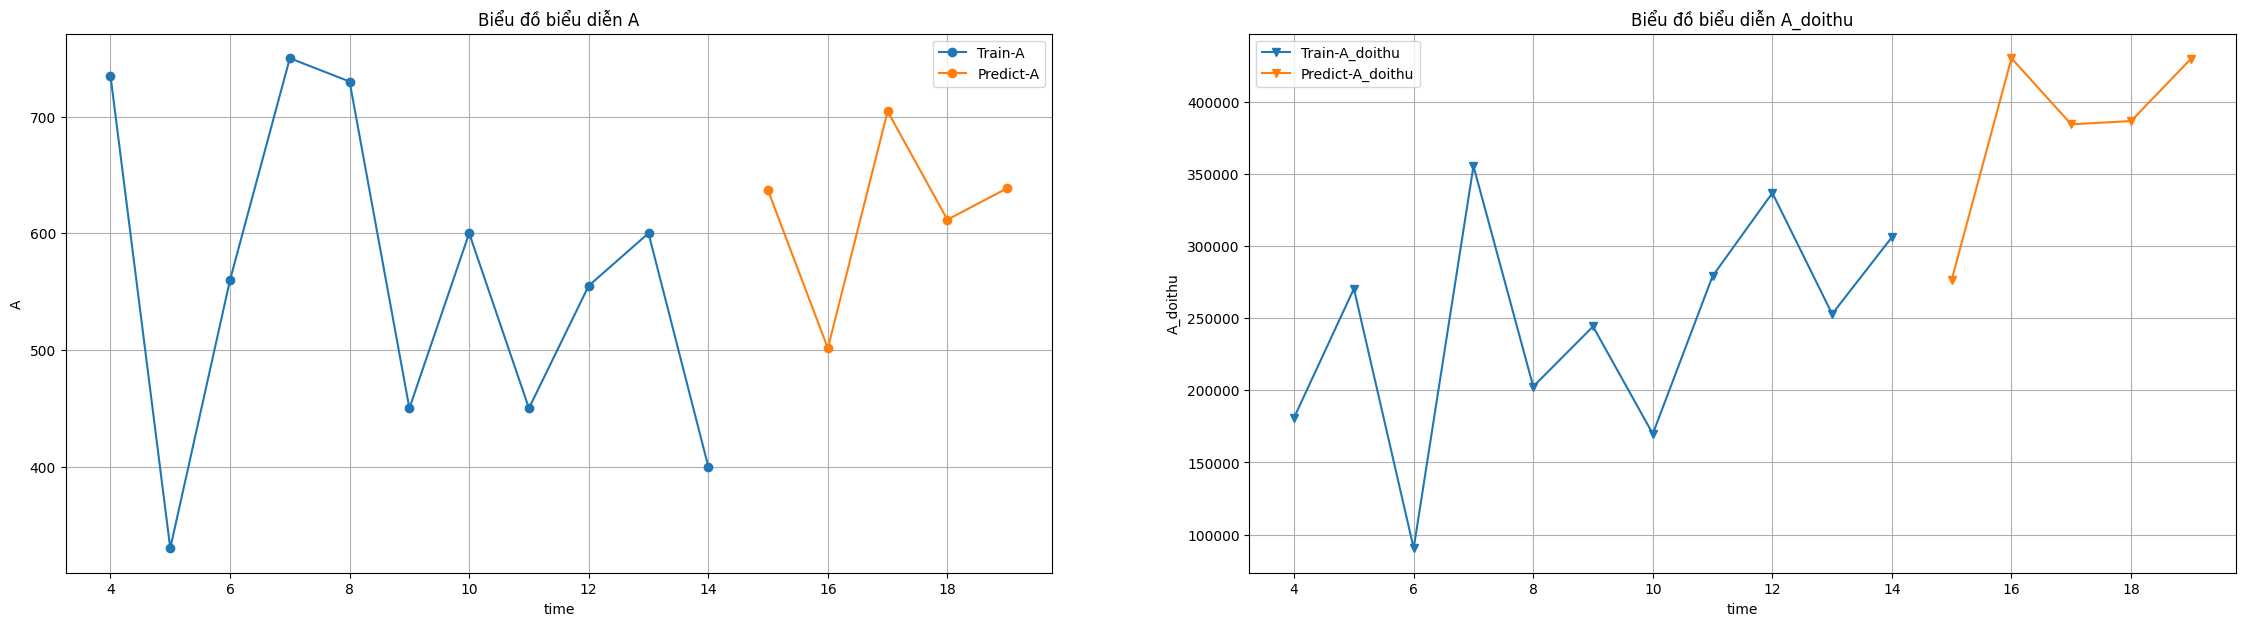
\includegraphics[width = \textwidth]{figure/VAR2.png}
    \caption{Dự đoán 4 quý năm 2024 của mô hình VAR - OLS trên 2 trường A và A đối thủ.}
    \label{fig:var2}
\end{figure}
\end{frame}


\begin{frame}{Mô hình VAR - OLS}
\begin{figure}[H]
    \centering
    \includegraphics[width = \textwidth]{figure/VAR3.png}
    \caption{Dự đoán 4 quý năm 2024 của mô hình VAR - OLS trên 3 trường B1, B2 và B đối thủ.}
    \label{fig:var2}
\end{figure}
\end{frame}

\begin{frame}{Mô hình VAR - OLS}
    \begin{figure}[H]
    \centering
    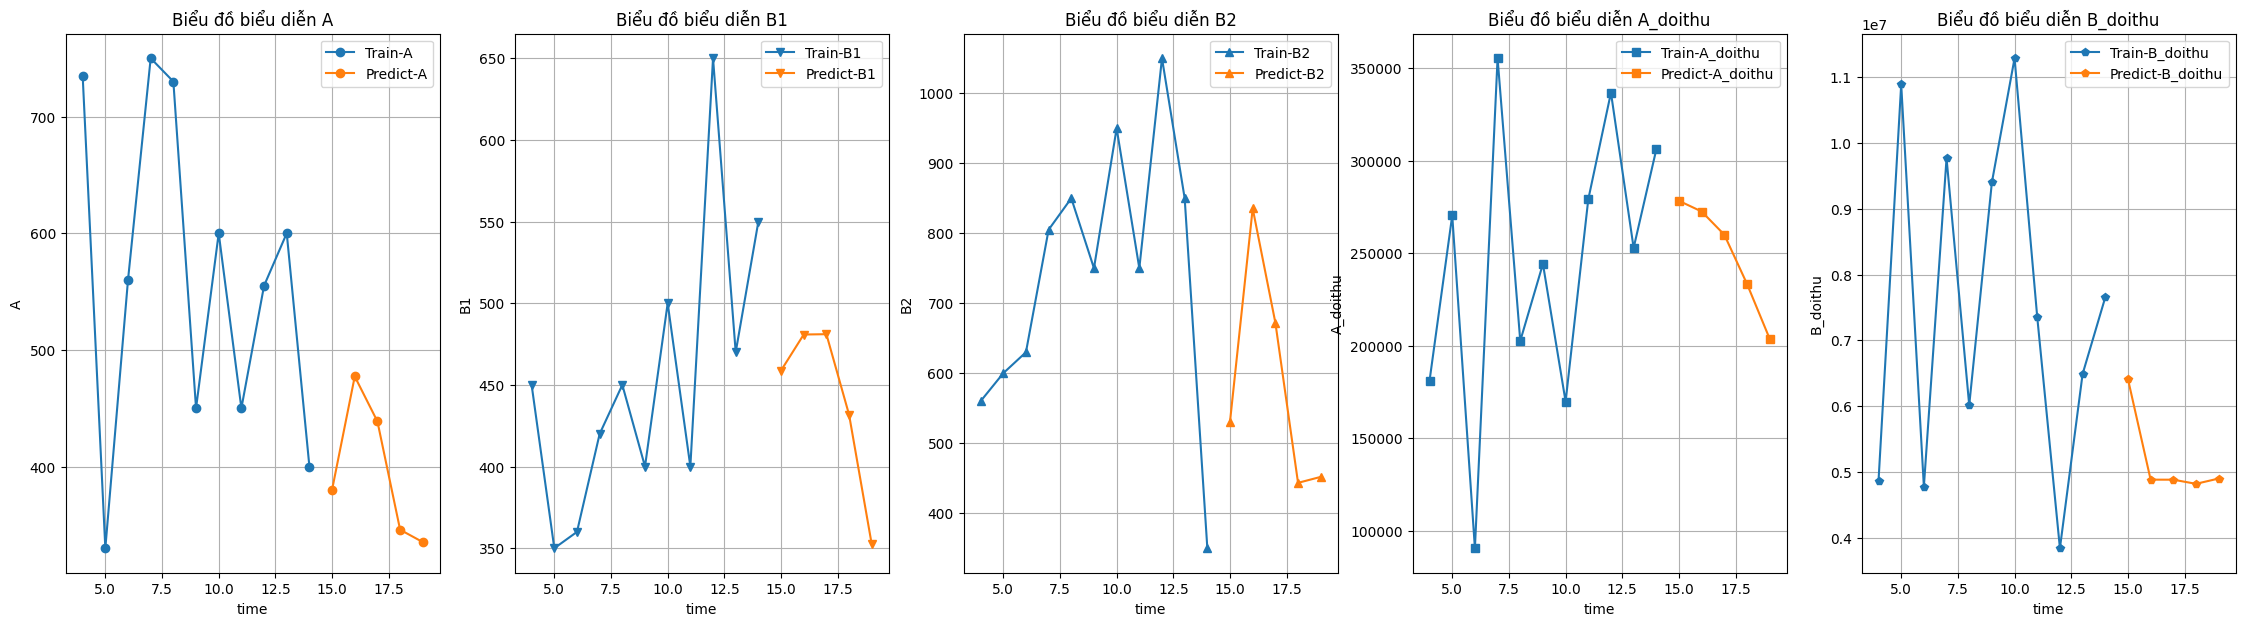
\includegraphics[width = \textwidth]{figure/dudoanVAR.png}
    \caption{Dự đoán 4 quý năm 2024 tiếp theo của mô hình VAR - OLS trên cả 5 trường.}
    \label{fig:var5}
\end{figure}
\end{frame}

\begin{frame}{Mô hình VAR - Durbin-Levinson}
    \begin{table}[H]
    \centering
    \caption{Kết quả dự báo 4 quý năm 2024 bằng mô hình VAR - Durbin-Levinson.}
    \label{DB4nam2024}
    \resizebox{\textwidth}{!}{ 
        \begin{tabular}{|c|c|c|c|c|c|c|c|c|c|c|}
        \hline
            \multirow{2}{*}{Quý} & \multicolumn{2}{c|}{A và A đối thủ} & \multicolumn{3}{c|}{B1, B2 và B đối thủ} & \multicolumn{5}{c|}{A, B1, B2, A đối thủ và B đối thủ} \\ \cline{2-11}
            & A & A đối thủ & B1 & B2  & B đối thủ & A & B1 & B2 & A đối thủ & B đối thủ \\ \hline
            1 & 534.637 & 260718.824 & 456.899 & 757.619 & 8020657.233 & 529.176 & 458.487 & 760.954 & 271257.466  & 7956737.484 \\ \hline
            2 & 572.094 & 236579.687 & 453.417 & 734.091 & 7291676.408 & 580.709 & 460.710 & 747.793 & 229189.165 & 7025864.153 \\ \hline
            3 & 554.189 & 248210.334 & 454.772 & 741.086 & 7565733.786 & 540.675 & 451.292 & 741.719 & 258889.882 & 7832721.811  \\ \hline
            4 & 562.794 & 242614.486 & 454.436 & 740.095 & 7451979.116 & 575.599 & 457.979 & 741.555 & 232923.170 & 7195879.347 \\ \hline
        \end{tabular}
    }
\end{table} 
\end{frame}

\begin{frame}{Mô hình VAR - Durbin-Levinson}
    \begin{figure}[H]
    \centering
    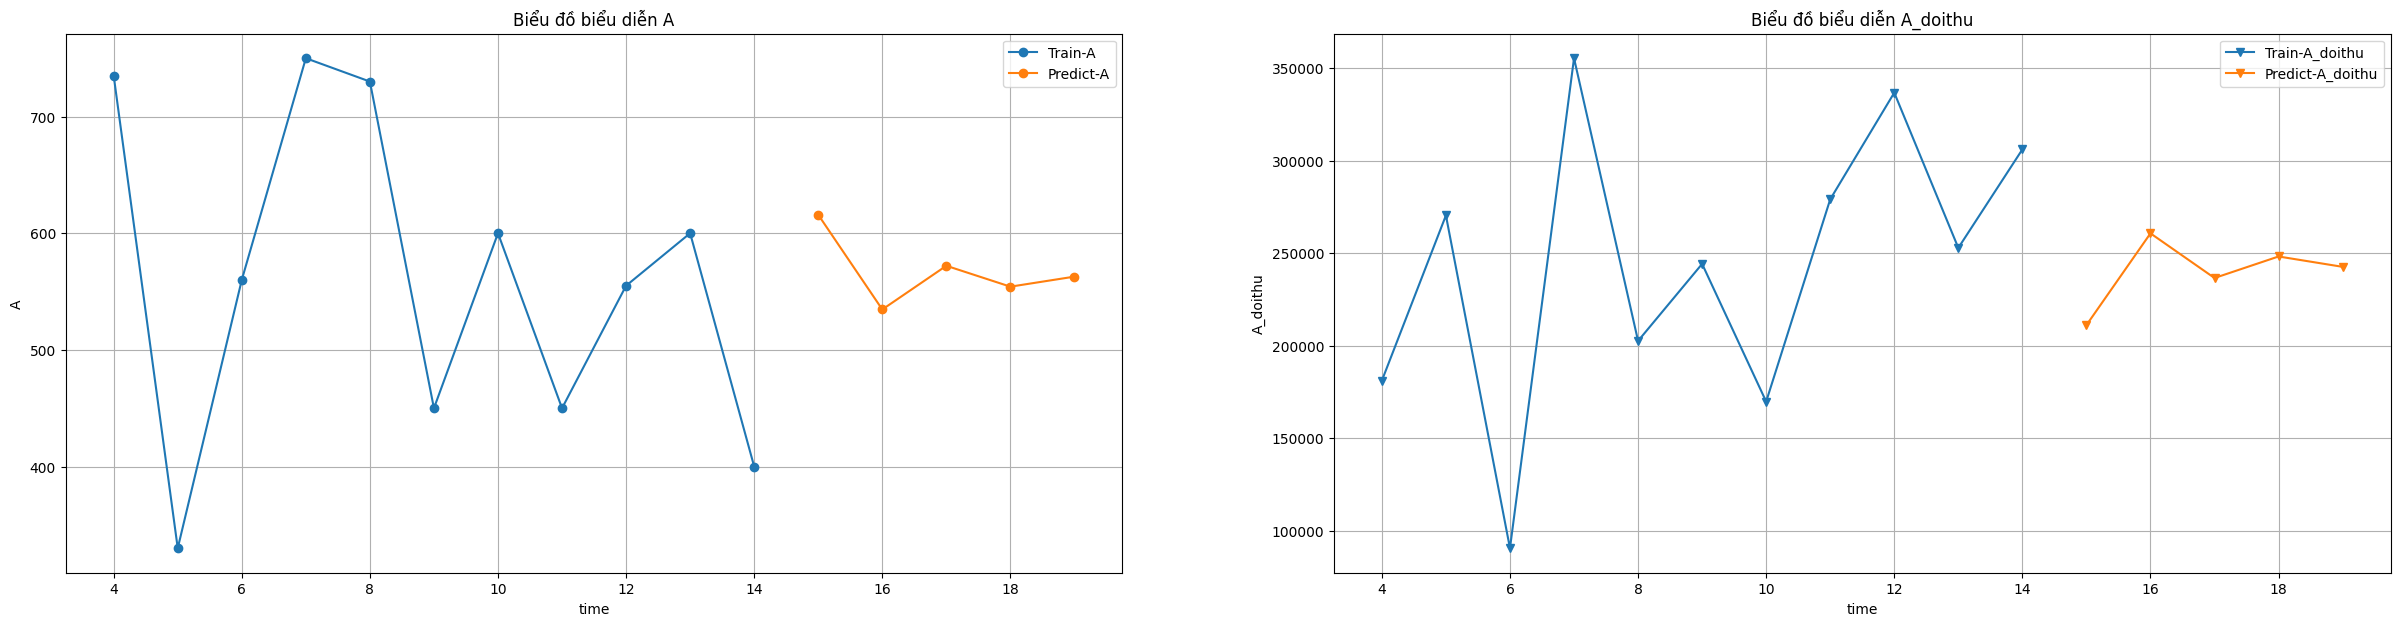
\includegraphics[width = \textwidth]{figure/preDB2.png}
     \caption{Kết quả dự đoán các quý tiếp theo của mô hình VAR - Durbin-Levinson trên 2 trường A và A đối thủ.}
\end{figure}
\end{frame}

\begin{frame}{Mô hình VAR - Durbin-Levinson}
    \begin{figure}[H]
    \centering
    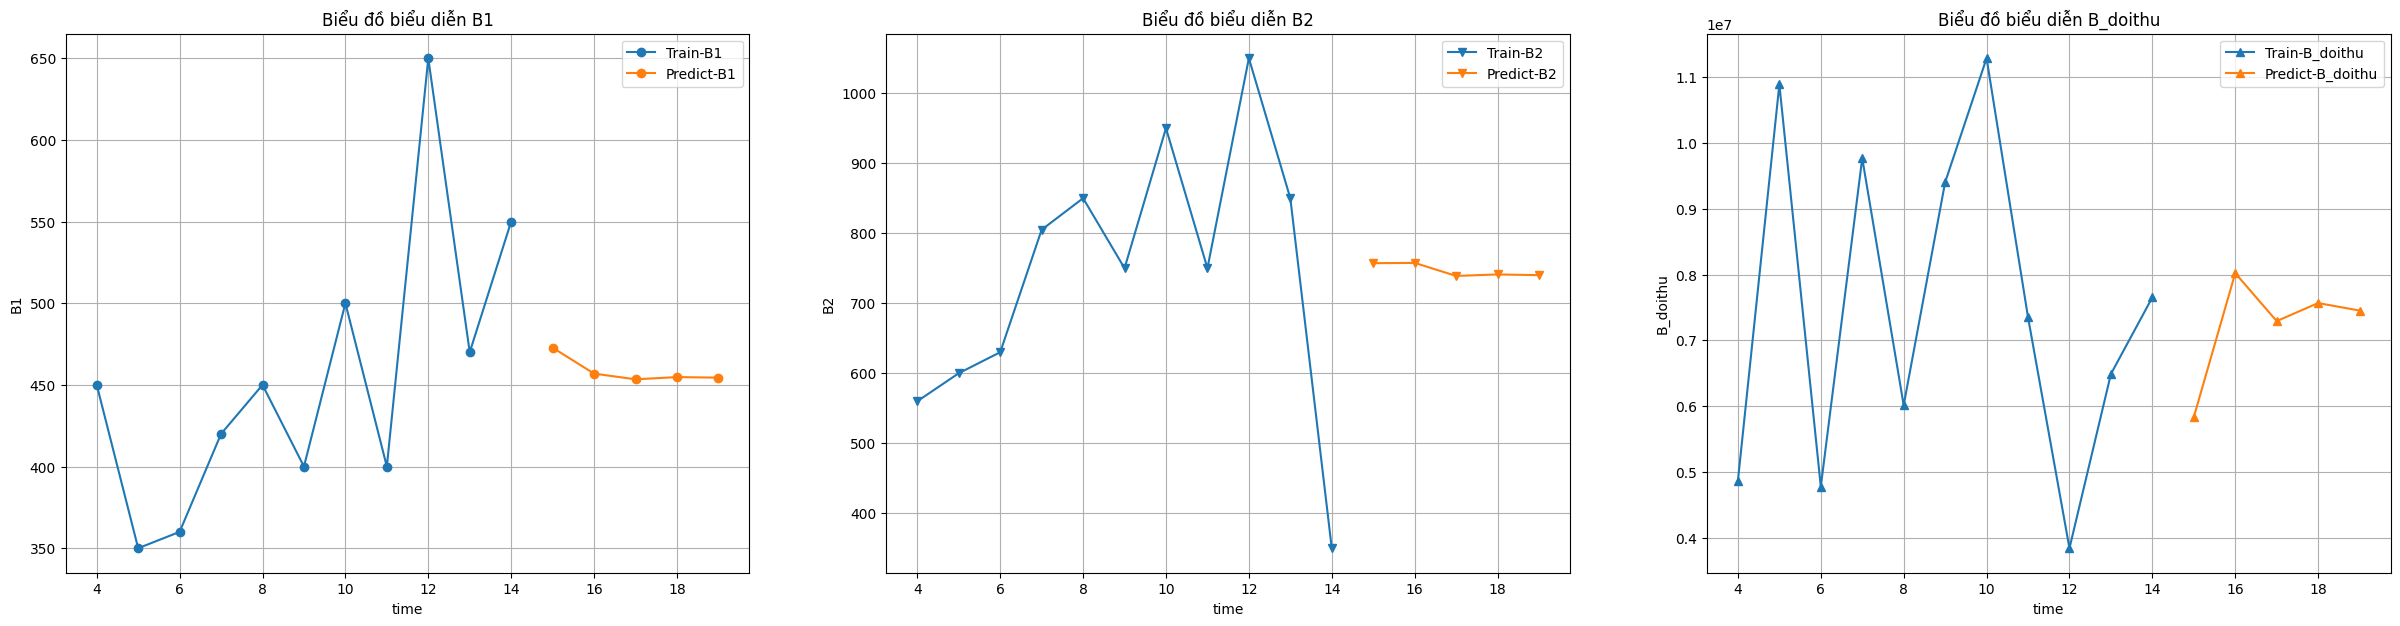
\includegraphics[width = \textwidth]{figure/preDB3.png}
     \caption{Kết quả dự đoán các quý tiếp theo của mô hình VAR - Durbin-Levinson trên 3 trường B1, B2 và B đối thủ.}
\end{figure}
\end{frame}

\begin{frame}{Mô hình VAR - Durbin-Levinson}
    \begin{figure}[H]
    \centering
    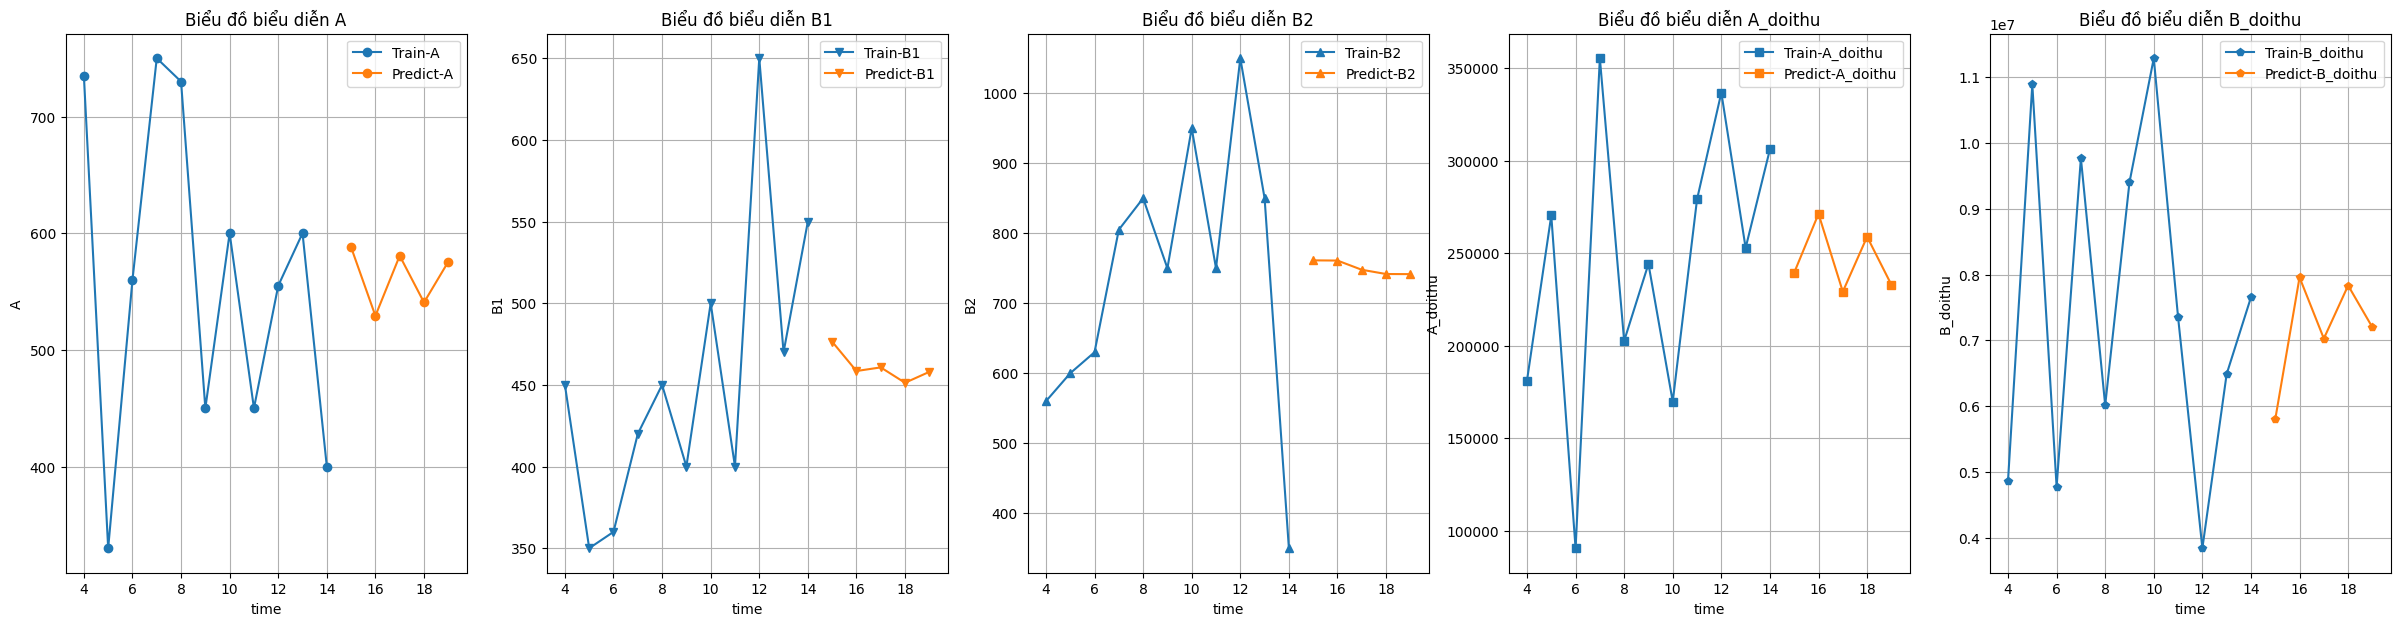
\includegraphics[width = \textwidth]{figure/preDB5.png}
     \caption{Kết quả dự đoán các quý tiếp theo của mô hình VAR - Durbin-Levinson trên cả 5 trường.}
\end{figure}
\end{frame}

\begin{frame}{Mô hình Holt-Winters tối ưu theo hàm Log-Likelihood}
    \begin{table}[H]
    \centering
    \caption{Kết quả dự báo 4 quý năm 2024 bằng mô hình Holt-Winters tối ưu theo hàm Log-Likelihood.}
    \label{HL4nam2024}
    \resizebox{\textwidth}{!}{ 
        \begin{tabular}{|c|c|c|c|c|c|}
        \hline
         Quý & A & B1 & B2 & A đối thủ & B đối thủ  \\ \hline
         1 & 611.179 & 667.743 & 945.461 & 337227.027 & 3748242.589 \\ \hline
         2 & 398.308 & 557.512 & 858.160 & 352909.032 & 7769289.737 \\ \hline
         3 & 458.769 & 620.615 & 767.525 & 285877.371 & 6748481.551 \\ \hline
         4 & 522.308 & 598.846 & 934.326 & 438602.865 & 7113320.903 \\ \hline
        \end{tabular}
    }
\end{table}
\end{frame}

\begin{frame}{Mô hình Holt-Winters tối ưu theo hàm Log-Likelihood}
    \begin{figure}[H]
    \centering
    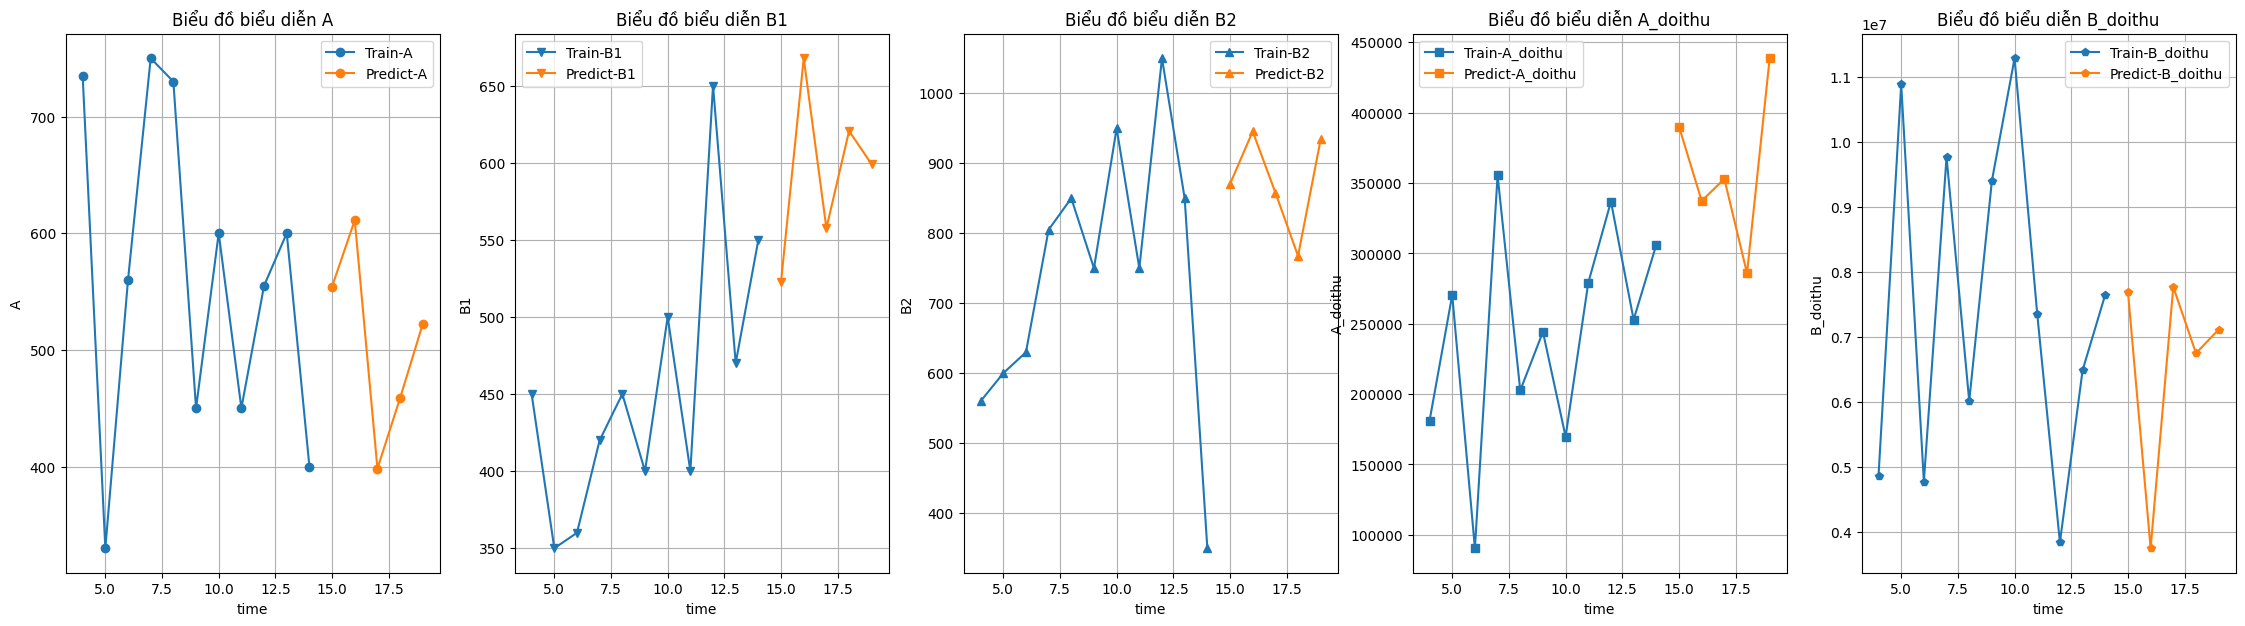
\includegraphics[width = \textwidth]{figure/HW-likelihood.png}
     \caption{Kết quả dự đoán 4 quý năm 2024 bằng mô hình Holt-Winters tối ưu theo hàm Likelihood.}
\end{figure}
\end{frame}

\begin{frame}{Mô hình Holt-Winters tối ưu theo hàm MSE}
    \begin{table}[H]
    \centering
    \caption{Kết quả dự báo 4 quý năm 2024 bằng mô hình Holt-Winters tối ưu theo hàm MSE.}
    \label{HM4nam2024}
    \resizebox{\textwidth}{!}{ 
        \begin{tabular}{|c|c|c|c|c|c|}
        \hline
         Quý & A & B1 & B2 & A đối thủ & B đối thủ  \\ \hline
         1 & 783.931 & 782.078 & 1181.535 & 408328.905 & 6563700.954 \\ \hline
         2 & 549.187 & 671.608 & 1103.708 & 431537.413 & 10697519.506 \\ \hline
         3 & 623.912 & 726.248 & 1034.390 & 354718.765 & 9344292.680 \\ \hline
         4 & 741.065 & 751.774 & 1263.108 & 541828.309 & 10713969.767 \\ \hline
        \end{tabular}
    }   
\end{table} 
\end{frame}

\begin{frame}{Mô hình Holt-Winters tối ưu theo hàm MSE}
    \begin{figure}[H]
    \centering
    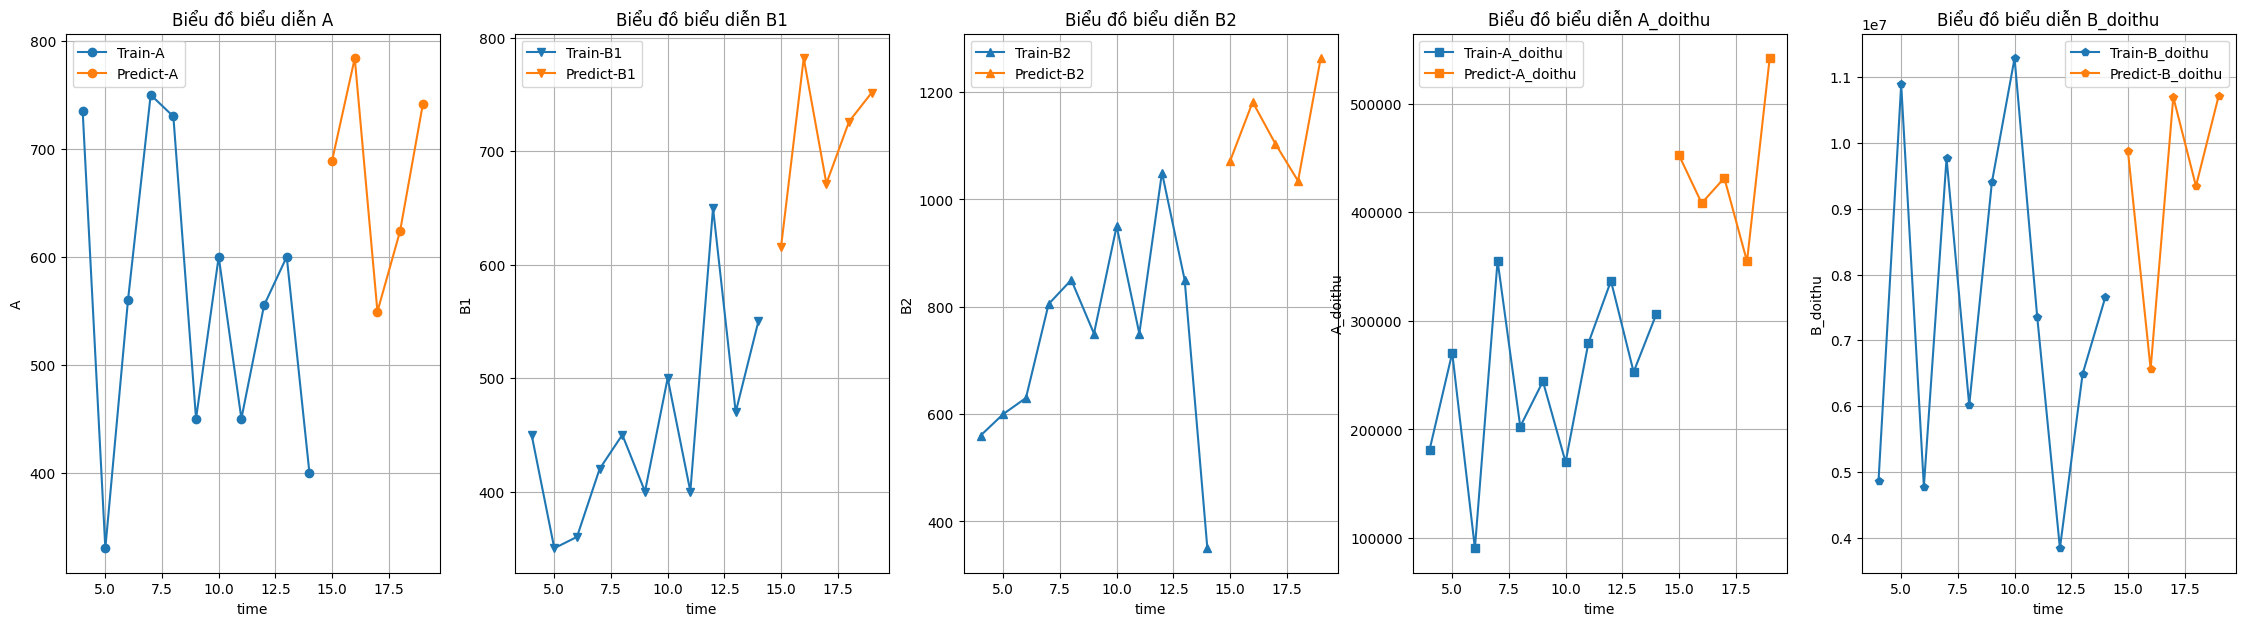
\includegraphics[width = \textwidth]{figure/HW-mse.png}
    \caption{Kết quả dự báo 4 quý năm 2024 bằng mô hình Holt-Winters tối ưu theo hàm MSE.}
\end{figure}
\end{frame}
\section{Kết luận}
\begin{frame}{Kết luận}
    Trong phạm vi nội dung của đồ án, một số nội dung mà nhóm chúng em đã đạt được:
\begin{itemize}
    \item Thành công trong việc giới thiệu 2 mô hình dự đoán chuỗi thời gian VAR và Holt-Winters. 
    \item Ứng dụng được vào bài toán dự báo nhu cầu sản phẩm.
    \item So sánh được hiệu quả của mô hình VAR và Holt-Winters trong bài toán dự báo nhu cầu sản phẩm.
\end{itemize}
Với những kết quả đạt được, đồ án có nhiều tiềm năng ứng dụng trong nhiều bài toán khác nhau về chuỗi thời gian. Một số hướng phát triển tiếp theo của đồ án:
\begin{itemize}
    \item Cải thiện độ chính xác của mô hình và ứng dụng vào nhiều lĩnh vực khác nhau, ví dụ: dự báo tỉ lệ người nhiễm covid, dự đoán doanh số bán hàng, v.v...
    \item Ứng dụng các mô hình học sâu để giải quyết bài toán.
\end{itemize}
\end{frame}
\end{footnotesize}
\begin{frame}{}
\centering
    \Huge{Thanks for listening!}
\end{frame}
\bibliographystyle{plain}
\bibliography{References.bib}   


\end{document}